\section{Apresentação}

Para apresentar os resultados será abordado tabelas contendo testes com todas combinações definidos nas \crefrange{tab:final_input_output_2d}{tab:final_output_2d_output_3d}.Em adição com a ilustração da última  execução de cada combinação representada na \cref{fig:result_final}.

\begin{table}[h]
            \centering
            \caption{Resultados dos testes entre imagem de entrada e mapa 2d}
            \label{tab:final_input_output_2d}
            \begin{tabular}{|c|c|c|c|c|c|c|c|}
                \hline
                                Pontos & IoU & Acc & F1 & MCC & FDR & FNR & Duração \\
                \hline
                50 & 0.71361 & 0.86085 & 0.8323 & 0.74079 & 0.2762 & 0.01923 & 5.33293\\
        100 & 0.80033 & 0.9151 & 0.88857 & 0.82809 & 0.17938 & 0.0292 & 10.0857\\
        150 & 0.83825 & 0.93506 & 0.91168 & 0.86398 & 0.13792 & 0.03125 & 15.32477\\
        200 & 0.85695 & 0.94434 & 0.92268 & 0.88059 & 0.10822 & 0.04269 & 20.22667\\
        250 & 0.868 & 0.94946 & 0.92908 & 0.89029 & 0.09454 & 0.04525 & 27.26459\\
        300 & 0.87405 & 0.95241 & 0.93263 & 0.89612 & 0.08326 & 0.04984 & 33.46705\\
                \hline
            \end{tabular}
        \end{table}


\begin{table}[h]
            \centering
            \caption{Resultados dos testes entre imagem de entrada e mapa de altura}
            \label{tab:final_input_output_3d}
            \begin{tabular}{|c|c|c|c|c|c|c|c|}
                \hline
                                Pontos & IoU & Acc & F1 & MCC & FDR & FNR & Duração \\
                \hline
                50 & 0.67955 & 0.83753 & 0.80827 & 0.70471 & 0.31036 & 0.02058 & 5.29547\\
        100 & 0.74929 & 0.88637 & 0.85581 & 0.77953 & 0.23518 & 0.02501 & 9.822\\
        150 & 0.79092 & 0.91133 & 0.88236 & 0.82054 & 0.18669 & 0.0319 & 15.43131\\
        200 & 0.80368 & 0.91818 & 0.89056 & 0.83234 & 0.17252 & 0.03302 & 21.06372\\
        250 & 0.82316 & 0.92831 & 0.90248 & 0.85016 & 0.14821 & 0.03784 & 25.92615\\
        300 & 0.82598 & 0.93022 & 0.90415 & 0.85286 & 0.14182 & 0.04223 & 32.75651\\
                \hline
            \end{tabular}
        \end{table}


\begin{table}[h]
            \centering
            \caption{Resultados dos testes entre mapa 2d e mapa de altura}
            \label{tab:final_output_2d_output_3d}
            \begin{tabular}{|c|c|c|c|c|c|c|c|}
                \hline
                                Pontos & IoU & Acc & F1 & MCC & FDR & FNR & Duração \\
                \hline
                50 & 0.91515 & 0.9589 & 0.95559 & 0.91721 & 0.06528 & 0.0222 & 5.0949\\
        100 & 0.90352 & 0.95708 & 0.94924 & 0.91312 & 0.08082 & 0.01838 & 10.08713\\
        150 & 0.90342 & 0.9592 & 0.94915 & 0.91636 & 0.08265 & 0.01631 & 14.82656\\
        200 & 0.90421 & 0.96087 & 0.94955 & 0.91901 & 0.08312 & 0.01487 & 20.51247\\
        250 & 0.90505 & 0.96207 & 0.95004 & 0.92088 & 0.08284 & 0.0142 & 26.63407\\
        300 & 0.90357 & 0.96252 & 0.94921 & 0.92112 & 0.08565 & 0.01276 & 33.59293\\
                \hline
            \end{tabular}
        \end{table}




\begin{figure}[!ht]
	\centering
    \caption{Resultados da última execução de cada combinação de imagens.}
	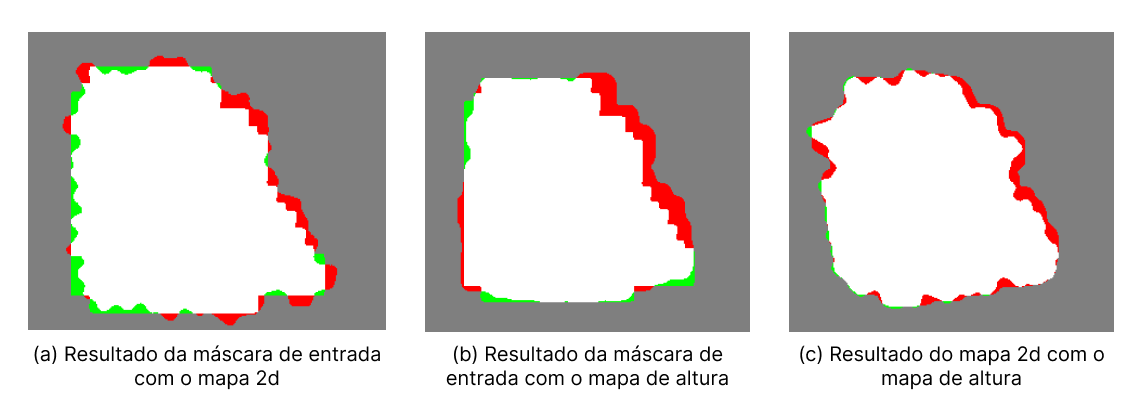
\includegraphics[width=\textwidth]{figures/comb_results_final.png}
    \legend{Fonte: \space Autoria própria}
	\label{fig:result_final}
\end{figure}

Na \cref{fig:combs_result} é demonstrado todos os passos contidios na execução do programa gerado em Python.

\begin{figure}[!ht]
	\centering
    \caption{Passos do programa final.}
	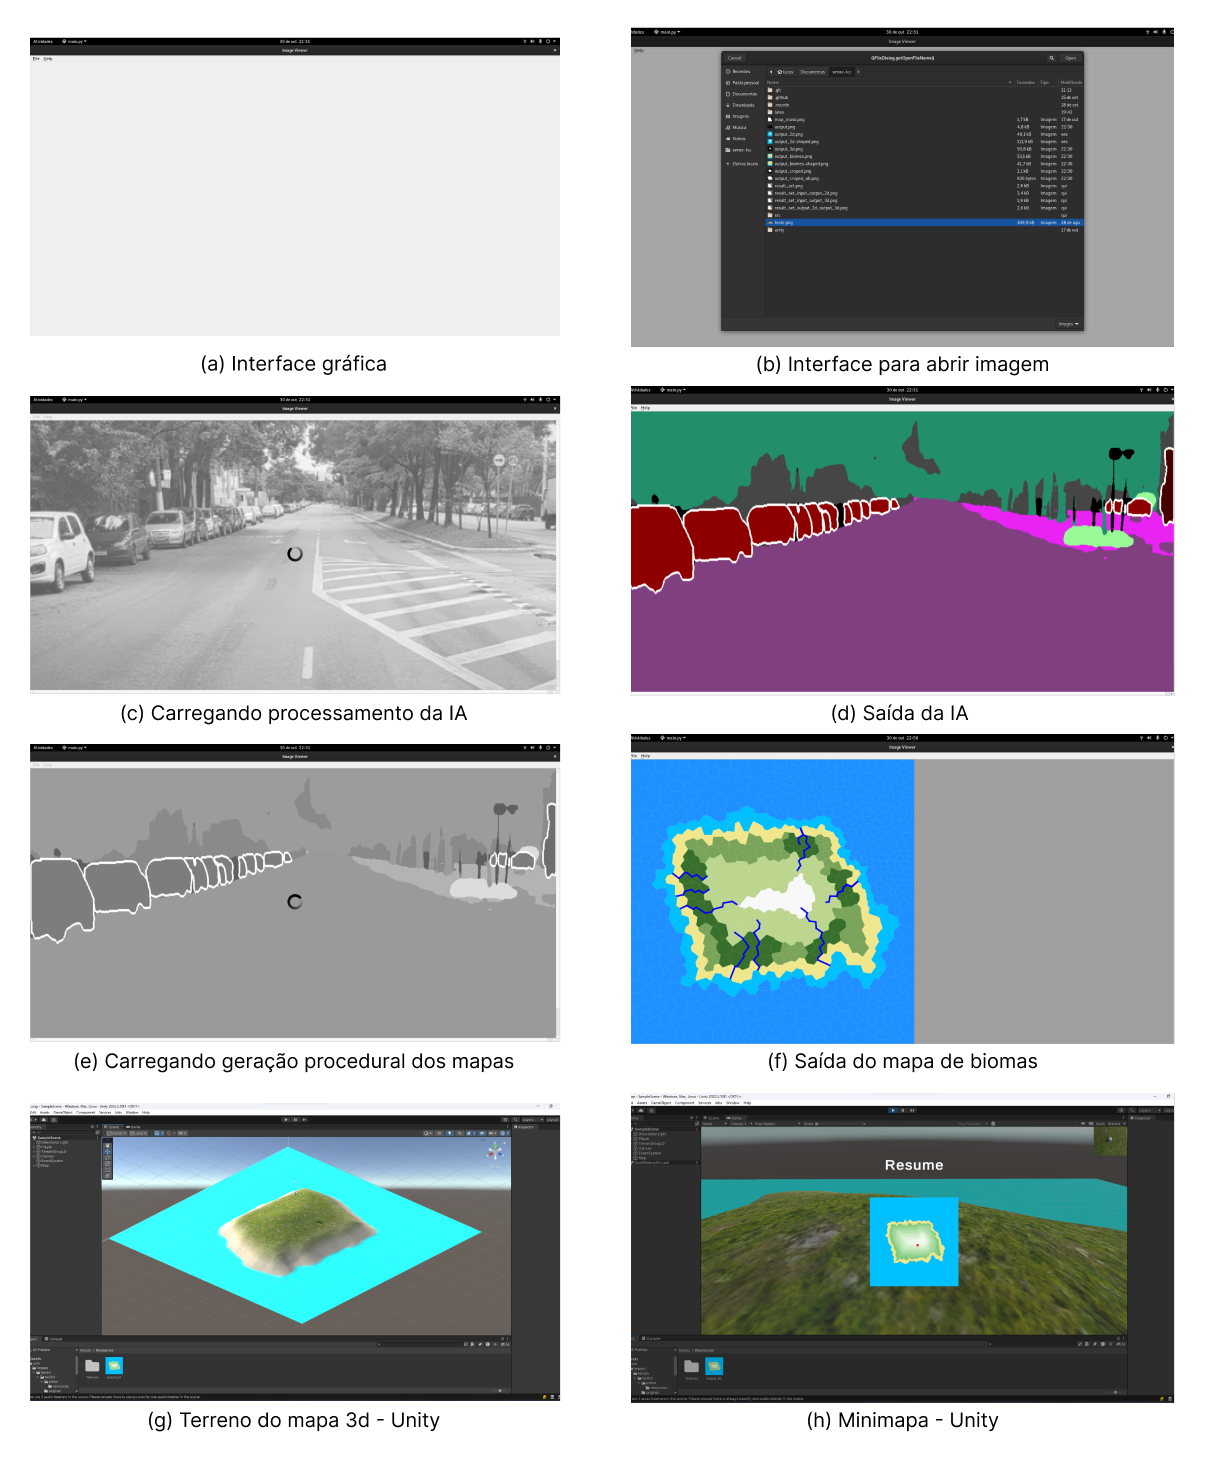
\includegraphics[width=\textwidth]{figures/result_final.png}
    \legend{Fonte: \space Autoria própria}
	\label{fig:combs_result}
\end{figure}